%%%%%%%%%%%%%%%%%%%%%%%%%%%%%%%%%%%%%%%%%
% Structured General Purpose Assignment
% LaTeX Template
%
% This template has been downloaded from:
% http://www.latextemplates.com
%
% Original author:
% Ted Pavlic (http://www.tedpavlic.com)
%
% Note:
% The \lipsum[#] commands throughout this template generate dummy text
% to fill the template out. These commands should all be removed when
% writing assignment content.
%
%%%%%%%%%%%%%%%%%%%%%%%%%%%%%%%%%%%%%%%%%

%----------------------------------------------------------------------------------------
%	PACKAGES AND OTHER DOCUMENT CONFIGURATIONS
%----------------------------------------------------------------------------------------

\documentclass{article}

\usepackage{fancyhdr} % Required for custom headers
\usepackage{lastpage} % Required to determine the last page for the footer
\usepackage{extramarks} % Required for headers and footers
\usepackage{graphicx} % Required to insert images
\usepackage{lipsum} % Used for inserting dummy 'Lorem ipsum' text into the template
\usepackage{natbib} % bibliography
\usepackage{filecontents}
\usepackage{pgfplots}
\usepackage{pgfplotstable}
\usepackage{siunitx}
\usepackage{float}
\usepackage{tikz}
\usepackage{tikz-uml}
\usetikzlibrary{backgrounds}
\pgfplotsset{compat=1.5}

% Margins
\topmargin=-0.45in
\evensidemargin=0in
\oddsidemargin=0in
\textwidth=6.5in
\textheight=9.0in
\headsep=0.25in

\linespread{1.1} % Line spacing

% Set up the header and footer
\pagestyle{fancy}
\lhead{\hmwkClass:\ \hmwkTitle} % Top left header
\chead{} % Top center header
\rhead{\firstxmark} % Top right header
\lfoot{\lastxmark} % Bottom left footer
\cfoot{} % Bottom center footer
\rfoot{Page\ \thepage\ of\ \pageref{LastPage}} % Bottom right footer
\renewcommand\headrulewidth{0.4pt} % Size of the header rule
\renewcommand\footrulewidth{0.4pt} % Size of the footer rule

\setlength\parindent{0pt} % Removes all indentation from paragraphs

%----------------------------------------------------------------------------------------
%	DOCUMENT STRUCTURE COMMANDS
%	Skip this unless you know what you're doing
%----------------------------------------------------------------------------------------

% Header and footer for when a page split occurs within a problem environment
\newcommand{\enterSectionHeader}[1]{
\nobreak\extramarks{#1}{#1 continued on next page\ldots}\nobreak
\nobreak\extramarks{#1 (continued)}{#1 continued on next page\ldots}\nobreak
}

% Header and footer for when a page split occurs between problem environments
\newcommand{\exitSectionHeader}[1]{
\nobreak\extramarks{#1 (continued)}{#1 continued on next page\ldots}\nobreak
\nobreak\extramarks{#1}{}\nobreak
}

\newcommand{\mainSectionName}{}
\newenvironment{mainSection}[1]{ % Makes a new environment called homeworkProblem which takes 1 argument (custom name) but the default is "Problem #"
\renewcommand{\mainSectionName}{#1} % Assign \homeworkProblemName the name of the problem
\section{\mainSectionName} % Make a section in the document with the custom problem count
\enterSectionHeader{\mainSectionName} % Header and footer within the environment
}{
\exitSectionHeader{\mainSectionName} % Header and footer after the environment
}

%----------------------------------------------------------------------------------------
%	NAME AND CLASS SECTION
%----------------------------------------------------------------------------------------

\newcommand{\hmwkTitle}{Market Chirp} % Assignment title
% \newcommand{\hmwkDueDate}{Monday,\ January\ 1,\ 2012} % Due date
\newcommand{\hmwkClass}{ABCs} % Course/class
\newcommand{\hmwkAuthorName}{Alex Fong, Brandon Woo, Chris Konstad, Sakib Shaikh} % Your name

%----------------------------------------------------------------------------------------
%	TITLE PAGE
%----------------------------------------------------------------------------------------

\title{
\vspace{2in}
\textmd{\textbf{\hmwkClass:\ \hmwkTitle}}\\
\vspace{3in}
}

\author{\textbf{\hmwkAuthorName}}
\date{December 3rd, 2015} % Insert date here if you want it to appear below your name

%----------------------------------------------------------------------------------------
% Bibliography
\begin{filecontents*}{ABCs.bib}
@MISC{GitBranching,
  author = {{Keith D. Gregory}},
  title = {{Practical Git: A Workflow to Preserve Your Sanity}},
  note = {[Online; accessed Nov 30, 2015]},
  url = {http://www.kdgregory.com/images/scm.git/02-fishbone.gif}
}
\end{filecontents*}
%------------------------------------------------------------------------------

%------------------------------------------------------------------------------
% USER ARRIVAL RATES
\begin{filecontents}{users.temp}
X,Y
0,1
30,2
60,4
90,8
120,16
150,32
180,64
210,128
240,256
270,512
\end{filecontents}
%------------------------------------------------------------------------------

\begin{document}

\maketitle

%----------------------------------------------------------------------------------------
%	TABLE OF CONTENTS
%----------------------------------------------------------------------------------------

%\setcounter{tocdepth}{1} % Uncomment this line if you don't want subsections listed in the ToC

\newpage
\tableofcontents
\newpage

%----------------------------------------------------------------------------------------
%	PROBLEM 1
%----------------------------------------------------------------------------------------

% To have just one problem per page, simply put a \clearpage after each problem

%\begin{homeworkProblem}
\begin{mainSection}{Introduction}
Market Chirp is a stock recommendation web application developed in the context of UCLA CS 188/219, Scalable Internet Services in Fall 2015 by the team ABCs. The application analyzes Twitter's sentiment on all NASDAQ stocks and provides the user with the information required to make sound investment decisions.
\\
\subsection{What we do} % TODO This should just be a statement, not an explanation
Market Chirp analyzes over 2,800 stocks in the New York Stock Exchange. Once a user creates an account, an aggregate of data appears in the dashboard. In the dashboard after selecting a stock, one can view the Twitter feed, the tweet sentiment of the stock, and the stock history. Common stock data such as the market cap and current versus historical stock price is gathered from Yahoo! Finance's API. In addition, Market Chirp takes a mix of the most influential and most recent tweets containing the current stock ticker's symbol of the past twenty-four hours and runs the tweets through a sentiment analyzer. The average of the sentiments is displayed along with a tweet that most closely matches the sentiment.
\\

In addition, one can favorite stocks to keep a running list of stocks to view with ease at later times. The favorited stocks appear in the sidebar and can be unfavorited at anytime.
\\
\begin{figure}[h]
  \centering
  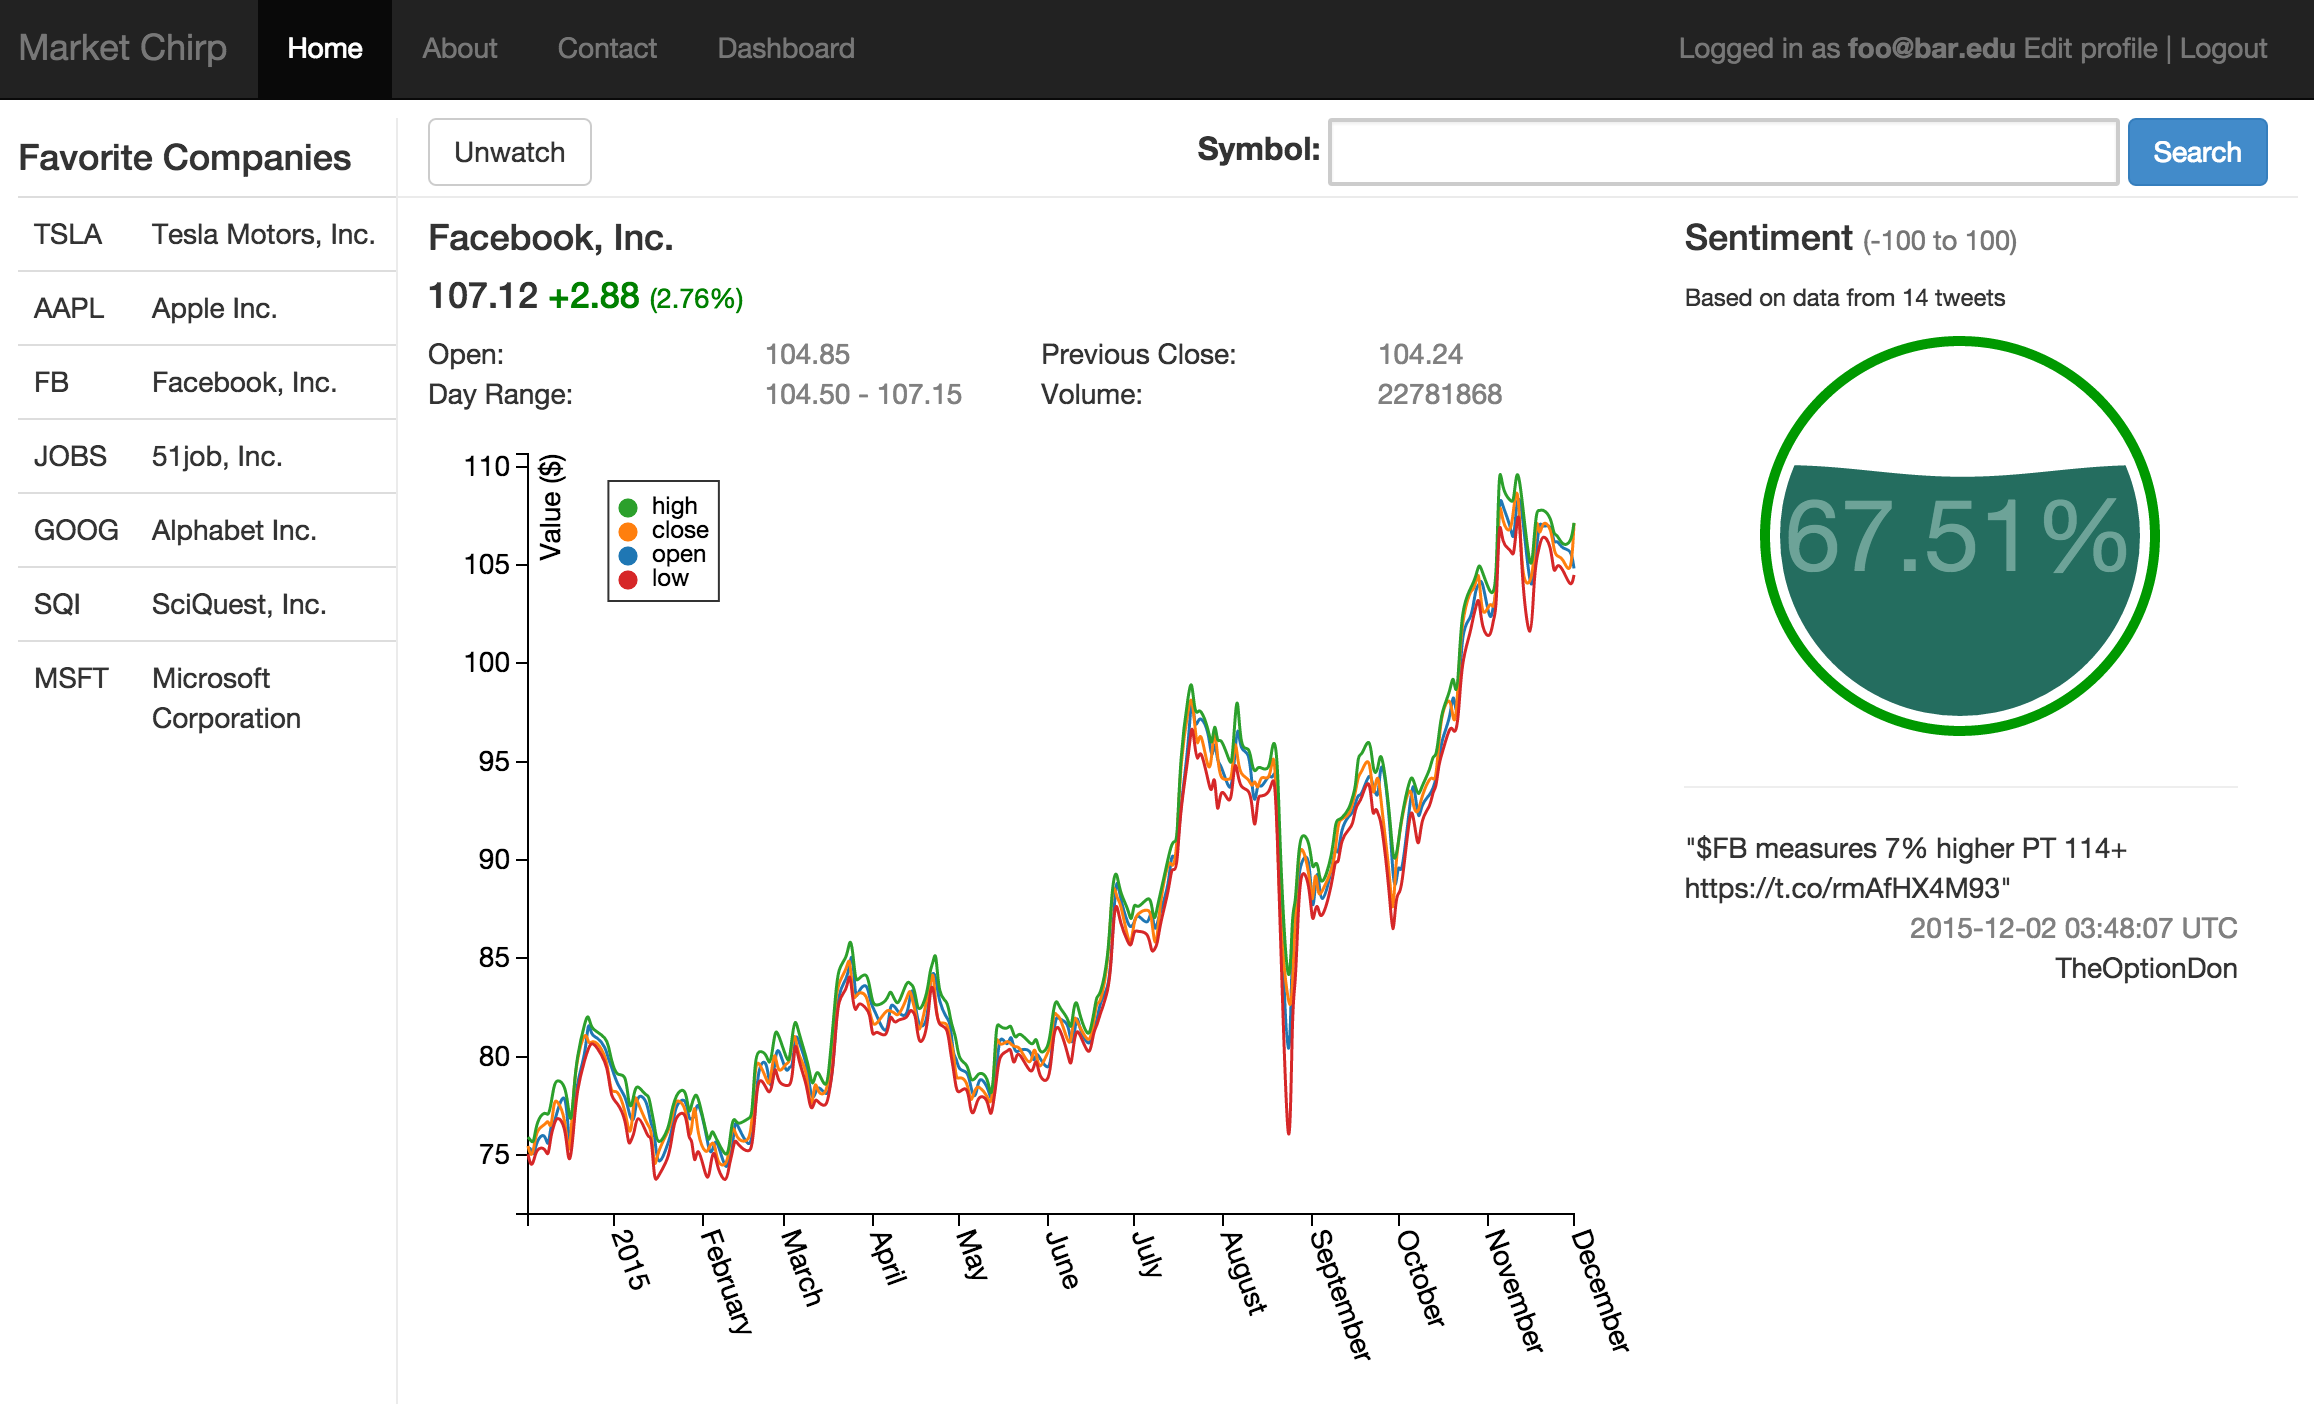
\includegraphics[width=1\columnwidth]{resources/dashboard.png} % Example image
  \caption{Example dashboard containing stock history, sentiment, and favorites.}
  \label{fig:dashboard}
\end{figure}
\subsection{Our goal}
The goal of Market Chirp is to quickly analyze the public's opinion of high-quality stocks through short notes on Twitter. Since the feed of Tweets is queried in real time when a user searches for a certain stock, the sentiment analysis of a stock is the public's current opinion of whether a stock is bullish or bearish. For example, if a stock's market price is on a downhill trend but its Twitter sentiment is on an uptrend, one may take that as an indication to buy the stock. This is because the temperature of a company in the eye of the public is often a good indicator of their stock's future performance on the market. Market Chirp's ultimate goal is not to predict the stock market as the sentiment is based on limited dataset of people tweeting about a stock, however it can give insight into the future of the stock based on public opinion.
\\
\subsection{How we do it}
Market Chirp is implemented in Ruby on Rails (Ruby 2.2.1 and Rails 4.2.4). The backend data store is a relational database management system, in our case MySQL. Since the purpose of CS 188/219: Scalable Internet Services is to build and deploy a scalable web service, this report will therefore discuss the deployment, performance and scalability of Market Chirp.
\end{mainSection}
\pagebreak

\begin{mainSection}{Development Process}
\begin{figure}[h]
  \centering
  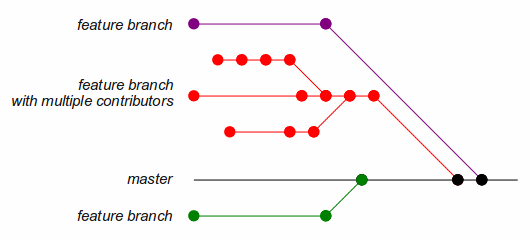
\includegraphics[width=0.75\columnwidth]{resources/git.jpg} % Example image
  \caption{Example of our Git branching technique (\cite{GitBranching})}
  \label{fig:git}
\end{figure}

\subsection{Planning}
Through the development of Market Chirp, our team used an Agile framework. Here we had weekly sprint planning meetings to discuss where the project was headed along with retrospective meetings to gain a perspective of what we had accomplished or still had yet to implement over the past week. Tasks not completed by the specified sprint date were automatically moved into a backlog or icebox in order to be completed in future sprints. By using these stand-up meetings, our team was able to precisely figure out the tasks that needed to be finished and how our individual features were pushed into the big picture of the entire product and its scalability.
\\

\subsection{Scheduling}
Pivotal Tracker guided us in following the Agile development framework. With Pivotal Tracker integrated with Github to keep track of certain features or issues, our commits and releases could be synced up to reflect the current status of the application. We were able to assign tickets to certain people in order to split the work up in an efficient manner. By modularizing the tasks, implementing the features and bug fixes was more smooth than using another development framework such as Waterfall Planning. As the quarter moved along however, our use of Pivotal Tracker slowly faded out as we kept in constant contact with each other and remained up to with our progress on the project.
\\

\subsection{Automated testing}
Since Rails is a test driven development framework, it automatically created testing templates for the classes we developed. We made sure to follow test driven development in which one creates test cases for a feature before actually implementing the feature. By following TDD, edge cases were covered as we programmed out the features since we were aware of them beforehand. Since we created ample test cases, the majority of our code was covered and allowed us to be confident our website would not crash when scaled upward.
\\

Travis CI was set up as a continuous integration service for building and testing project. We created numerous test cases that would be run each commit to see the version control's reliability. Connecting Travis CI to Github allowed us to keep commiting new code and test its reliability and keep it bug free.
\\

To further minimize the bugs in our code and to follow the D.R.Y. practices, we ran Rubocop and Pre-commit before our commits. Rubocop is a Ruby static code analyzer that enforces many of the guidelines outlined in the community Ruby Style Guide. This linter analyzed all of the code in our repository and provided metrics that ensured our Ruby code was stylistically intact. Before we committed our code, Git fired off a pre-commit hook that ran Rubocop. If Rubocop returned any warnings on our code, our code could not be committed. Thus, our code was ensured to be up-to-date with the current stylistic guidlines.
\\
\subsection{Version control}
Our version control management system was Git. By keeping the master branch as our production branch, our releases on AWS were always in sync with the latest release on our remote Github. We all worked on separate branches and used pull requests to merge our new code into the other branches eventually merging into master. Through constant rebasing of our branches, we were able to keep our development history clean and appear as though only one person had developed it. Separating the features and bug fixes into their own respective branch allowed each developer to focus on his own feature without conflicting with other developers. After merging in any new features, our application's version control history remained clean.
\\

\subsection{Pair programming}
Another development strategy we made use of was pair programming. This was true during the development of our Memcached server side caching optimization as well as during the implementation of Ruby's devise gem for logins. Pair programming allowed us to minimize the errors in our code since we had multiple eyes on the screen at a time. One person could focus on hashing out the code while the other checked for syntactic or logical errors. In doing so, the time from the outlining of a feature to pushing production ready code was optimized and we were able to save a substantial amount of time.
\\
\end{mainSection}

\begin{mainSection}{Application Architecture}
  Ruby on Rails' use of a MVC (Model View Controller) system allowed us to quickly prototype features during development, and later provided insulation between different aspects of our website. The user facing View provides the graphical interface with which they can see the result of their actions. When the user wants to interact with the application, say by submitting a form or searching for a stock, they are using a Controller. Lastly there is the Model which takes instructions from the Controller and updates the user's View. The Model also interacts with our application's database, in our case by keeping track of favorite stocks and cached data.
\\

\end{mainSection}
\pagebreak

\begin{mainSection}{Architecture}
  \subsection{Database layout}
  \begin{figure}[H]
    \begin{tikzpicture}
      % COMPANY
      \begin{umlclass}[x=5,y=5]{Company}{symbol : varchar(5)\\name : varchar(255)\\sector : varchar(255)\\industry : varchar(255)\\created\_at : datetime\\updated\_at : datetime\\
        }{}
      \end{umlclass}
      % FAVORITE_COMPANY
      \begin{umlclass}[x=0,y=0]{Favorite\_Company}{user\_id : foreign\_key\\company\_id : foreign\_key\\active : boolean\\created\_at : datetime\\updated\_at : datetime
        }{}
      \end{umlclass}
      % USER
      \begin{umlclass}[x=11,y=0]{User}{email : varchar(255)\\encrypted\_password : varchar(255)\\reset\_password\_token : varchar(255)\\reset\_password\_sent\_at : datetime\\remember\_created\_at : datetime\\sign\_in\_count : int(4)\\current\_sign\_in\_at : datetime\\last\_sign\_in\_at : datetime\\current\_sign\_in\_ip : varchar(255)\\last\_sign\_in\_ip : varchar(255)\\created\_at : datetime\\updated\_at : datetime
        }{}
      \end{umlclass}
      % FINANCE_CACHE
      \begin{umlclass}[x=0,y=10]{Finance\_Cache}{hist\_data : varchar(65535)\\curr\_data : varchar(65535)\\category : int(4)\\company\_id : foreign\_key\\created\_at : datetime\\updated\_at : datetime
        }{}
      \end{umlclass}
      % SENTIMENT_CACHE
      \begin{umlclass}[x=11,y=10]{Sentiment\_Cache}{tweet\_when : datetime\\score : decimal\\tweet\_text : varchar(255)\\tweet\_author : varchar(255)\\num\_tweets : int(4)\\company\_id : foreign\_key\\created\_at : datetime\\updated\_at : datetime
        }{}
      \end{umlclass}
      \umluniassoc[geometry=|-|]{Company}{Favorite\_Company}
      \umluniassoc[geometry=|-|]{Finance\_Cache}{Company}
      \umluniassoc[geometry=|-]{Sentiment\_Cache}{Company}
      \umluniassoc[geometry=|-|]{User}{Favorite\_Company}
    \end{tikzpicture}
    \caption{Diagram of the database tables and how they are connected.}
    \label{fig:database_layout}
  \end{figure}
\end{mainSection}

\begin{mainSection}{Testing}
  \subsection{Server configuration}
  We used the following software packages for the deployment of the production version of our application:
  \begin{itemize}
    \item Nginx
    \item Phusion Passenger
    \item MySQL
  \end{itemize}

  We modified the provided cloud formation template's JavaScript Object Notation (JSON) files to configure our server with the proper environmental variables, letting us keep our secret keys out of our public version control.\\

  The service was developed on our personal laptops, with all performance testing running on Amazon Web Services (AWS).  It was trivial for us to deploy new versions because we only had to deploy for performance testing, which was handled by our server provisioning scripts.\\

\begin{figure}[H]
  \begin{center}
    \begin{tabular}{| l | r | r | r | }
      \hline
      \multicolumn{4}{ |c| }{M3 Server Configurations}\\
      \hline
      Server Size & Cores & RAM (GiB) & Process Parallelization\\
      \hline
      Med     & 1 &  3.75 & 1 \\
      Large   & 2 &  7.50 & 2 \\
      XLarge  & 4 & 15.00 & 4 \\
      2XLarge & 8 & 30.00 & 8 \\
      \hline
    \end{tabular}
    \caption{Table of server configurations.  These settings were used for all tests.  For a server with $n$ cores, $n$ worker processes were used.  Each worker process was single threaded. By minimizing differences in the testing setups, we were able to clearly show the effects of each optimization.}
    \label{tab:m3}
  \end{center}
\end{figure}

When separate database servers were used (for example, in horizontal scaling), the database server was the same size as the application server (\texttt{db.m3med} was used for \texttt{m3.med}).\\

After analyzing our common queries, we added indicies to our database to improve read performance.  These indicies reduced query time for reads, improving database performance for our most common operation.\\

  \subsection{User simulation}
  \begin{figure}[H]
    \begin{center}
      \begin{tikzpicture}
        \begin{axis}[title=Test User Arrival Rates,
            xlabel = Time (sec),
            ylabel = Users/sec,
            legend pos = outer north east,
          ]
          \addplot[thick, orange] table [
              col sep=comma,
              x = X,
              y = Y,
            ] {users.temp};
        \end{axis}
      \end{tikzpicture}
    \end{center}
    \caption{Graph showing the number of test users sent from our Tsung server to our application server throughout the duration of the performance tests.}
    \label{graph:users}
  \end{figure}

  Our Tsung tests used the test user arrival rates shown in Figure \ref{graph:users}. A tabulation of the phases of users arrival rates can be seen below.\\

\begin{figure}[H]
  \begin{center}
    \begin{tabular}{| c | c | c | c | c | c | c | c | c | c | c |}
      \hline
      \multicolumn{11}{ |c| }{10 Phases of user arrivals}\\
      \hline
       Phase Number & 1 & 2 & 3 & 4 & 5 & 6 & 7 & 8 & 9 & 10\\
      \hline
      New users per second & 1 & 2 & 4 & 8 & 16 & 32 & 64 & 128 & 256 & 512\\
      \hline
    \end{tabular}
  \end{center}
  \caption{Table listing the number of users arriving per second during each phase of the test.}
\end{figure}

  Missing our slowest level of caching, our MySQL "caches" of Twitter sentiment data, and to a lesser extent Yahoo! Finance data, causes $20+$ second delays.  Because of these unreasonably long delays, our service would have worker processes keeping those caches warm if we deployed this to the real world.  To simulate this effect in our tests, we limited our test users to interacting with a small subset of the real world stocks and we warmed up the cache before running the tests.  According to our tests, users only care about Apple, Facebook, Google and Tesla stocks, which, while unrealistic, is a useful simulation for comparing performance tests.  Another benefit of focusing on popular stocks is that we are guaranteed to always have enough Twitter data about each stock symbol.  Some of the less popular stock symbols would have 5 tweets or less, making both the data inaccurate and the request too easy to strain the system.\\


  \subsection{Critical Path}
  Our critical path through our application was the path that we thought the average user was most likely to hit.  We had two user models, with a 50\% chance that either model was selected for each test user:
  \begin{enumerate}
    \item A user who is not logged in
    \item A user who is logged in
  \end{enumerate}

  While visiting each page, the test user would wait a randomized amount of time up to a threshold to emulate a person either looking at the page or filling out forms.

  \subsubsection{User not logged in}
  A user who is not logged in has no account on Market Chirp and therefore has no favorites.  They are also unable to access the Dashboard feature, which is the page that requires the most data fetching and handling, making it the most expensive page to load.  Instead, this user:
  \begin{enumerate}
    \item Visits our homepage
    \item Visits our sentiment analysis page
    \item Searchs for FB
    \item Searches for AAPL
    \item Searches for GOOGL
    \item Searches for TSLA
    \item Visits our stock data page
    \item Searchs for FB
    \item Searches for AAPL
    \item Searches for GOOGL
    \item Searches for TSLA
  \end{enumerate}

  \subsubsection{User is logged in}
  A logged in user would want to check their favorited stocks, which is most easily done through the Dashboard page.  From there, we thought the average user would check their stocks, look for a new one, favorite the new stock and drop one of their favorited stocks.  This user:
  \begin{enumerate}
    \item Logs in
    \item Visits their dashboard
    \item Visits the dashboard for GOOGL
    \item Favorites GOOGL
    \item Visits the dashboard for TLSA
    \item Visits the dashboard for FB
    \item Visits the dashboard for AAPL
    \item Removes AAPL from their favorite list
    \item Logs out
  \end{enumerate}

  \subsection{Initial testing}
  The first tests of Market Chirp showed massive performance issues.  Twitter sentiment data was calculated for all 100 tweets (pulled from Twitter separately for each request), leading to $20+$ second delays in getting results when searching for a stock symbol.  From looking at the logs and \texttt{top}, it was clear that the process was CPU bound.  No formal Tsung testing happened at this performance level because individual page loadings took too long and the service was not ready for even a single user.\\

  A MySQL driven "cache" was created to store Twitter analysis data for a day, for each stock that was searched.  While initial stock searches caused unreasonable delays of $20+$ seconds, subsequent delays were much, much faster, happening in less than $5$ seconds.  The cache stores the overall calculated sentiment and it stores a single tweet out of the $100$ sampled tweets that has the closest sentiment value as an average tweet for the given sample.\\

  A similar MySQL driven caching system as added to cache the 10 years of Yahoo! Finance stock data downloaded for each symbol requested.  The stock data itself was stored as a JSON text blob, as the client side graphing library read in that JSON.  It made more sense to store the JSON received from Yahoo! Finance in the same format that the graph required, than it did to parse the JSON, store each value individually, and read those values out as JSON later.

  \subsection{Vertical scaling}
  Vertical scaling, simply throwing more processing power at the problem, is simple but expensive.  We expected to get marginal performance gains by scaling vertically because our main bottleneck was the CPU bound Twitter sentiment analysis.

  \begin{figure}[H]
    \begin{center}
      \begin{tikzpicture}
        \begin{axis}[title=Vertical Scaling,
            xlabel = Time (sec),
            ylabel = 200 users/sec,
            legend pos = outer north east,
          ]
          \addplot[thick, orange] table [
              col sep=comma,
              x = X,
              y = Y,
            ] {resources/m3med/data/200.csv};
          \addplot[thick, blue] table [
              col sep=comma,
              x = X,
              y = Y,
            ] {resources/m3large/data/200.csv};
          \addplot[thick, green] table [
              col sep=comma,
              x = X,
              y = Y,
            ] {resources/m3xlarge/data/200.csv};
          \addplot[thick, magenta] table [
              col sep=comma,
              x = X,
              y = Y,
            ] {resources/m32xlarge/data/200.csv};
          \addlegendentry{M3 Med}
          \addlegendentry{M3 Large}
          \addlegendentry{M3 XLarge}
          \addlegendentry{M3 2XLarge}
          \end{axis}
        \end{tikzpicture}
      \end{center}
      \caption{Graph of performance during vertical scaling.}
      \label{graph:vertical}
    \end{figure}

    Figure \ref{graph:vertical} shows the result of our vertical scaling. As expected, when double the processing power was thrown at the problem, the number of users processed per second roughly doubled.

  \subsection{Horizontal scaling}
  For horizontal scaling, we moved from a single server that handled both the application server and the database to a network of servers (Figure \ref{graph:horizontal}).  This network contained an elastic load balancer (LB), two application servers (S0 and S1) and a MySQL server (DB).  This is a fairly standard horizontal scaling technique that makes it easy to increase the number of application servers dynamically (a side benefit of this is that each application server can be small, cheap, and unreliable as a new server can be spun up to take its place if it fails).
  \begin{figure}[H]
    \begin{center}
      \begin{tikzpicture}
        \begin{axis}[title=Horizontal Scaling,
            xlabel = Time (sec),
            ylabel = 200 users/sec,
            legend pos = outer north east,
          ]
          \addplot[thick, orange] table [
              col sep=comma,
              x = X,
              y = Y,
            ] {resources/multi_m3med/data/200.csv};
          \addplot[thick, blue] table [
              col sep=comma,
              x = X,
              y = Y,
            ] {resources/multi_m3large/data/200.csv};
          \addplot[thick, green] table [
              col sep=comma,
              x = X,
              y = Y,
            ] {resources/multi_m3xlarge/data/200.csv};
          \addplot[thick, magenta] table [
              col sep=comma,
              x = X,
              y = Y,
            ] {resources/multi_m32xlarge/data/200.csv};
          \addlegendentry{M3 Med}
          \addlegendentry{M3 Large}
          \addlegendentry{M3 XLarge}
          \addlegendentry{M3 2XLarge}
          \end{axis}
        \end{tikzpicture}
      \end{center}
      \caption{Graph of performance during horizontal scaling.}
      \label{graph:horizontal}
    \end{figure}
    Figure \ref{graph:horizontal} shows the result of our horizontal scaling. As expected, when double the amount of servers were thrown at the problem, the number of users processed per second doubled.  Unlike vertical scaling, horizontal scaling is essentially limitless, and is usually cheaper.

    \begin{figure}[H]
      \begin{center}
        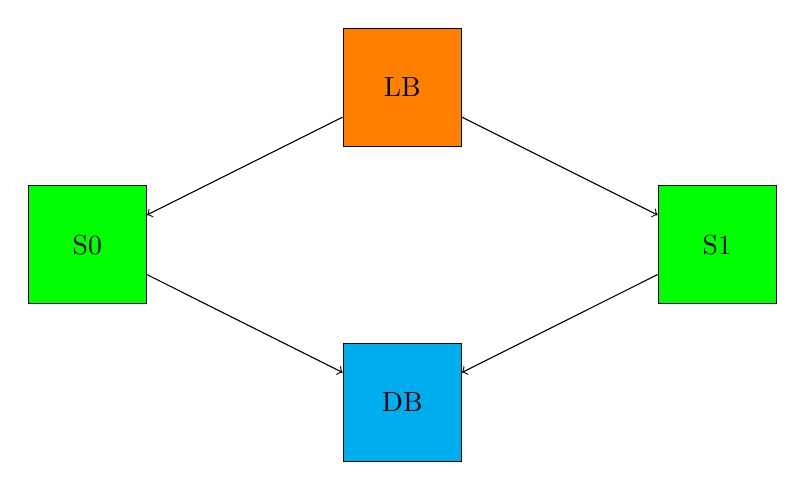
\begin{tikzpicture}[every node/.style={rectangle, fill=green,minimum width=15mm, minimum height=15mm,draw}]
          \node[fill=orange] (lb) at (0,0) {LB};
          \node (s0) at (-4,-2) {S0};
          \node (s1) at (4,-2) {S1};
          \node[fill=cyan] (db) at (0,-4) {DB};

          \begin{scope}[on background layer]
            \draw[->] (lb) edge (s0);
            \draw[->] (lb) edge (s1);
            \draw[->] (s0) edge (db);
            \draw[->] (s1) edge (db);
          \end{scope}
        \end{tikzpicture}
      \end{center}
      \caption{Network of Load Balancer, Servers, and Database Server}
      \label{dig:horizontal}
    \end{figure}
    Figure \ref{dig:horizontal} shows the configuration of our load balancer, servers and database.  This method of scaling lets us easily add more application servers to increase our available processing power, while not having to deal with distributed databases or more complex data persistence layers (although we are able to improve the data persistence layer if we want).\\

    We expect our database to be mostly read, with much fewer writes as users are likely to spend more of their time accessing stock data than they are favoriting or unfavoriting stocks.  Therefore, if we wanted to increase the performance of our data persistence layer, we would add read-only slaves with a write-master.  However, as seen in Section \ref{subsec:mem}, moving to Memcached eliminated the need for our MySQL database to cache the stock analysis and price data, reducing database hits.

  \subsection{In-memory caching} \label{subsec:mem}
  Another method we implemented to speed up our application was to use a memory object caching system. We used Memcached in our application through the \texttt{dalli} gem, which stores the cache in memory instead of on disk. Since memory provides faster access times than disk, the read and write times of cache fragments were reduced. In order to provide this server-side caching, a new instance of Memcached needed to be started within each server. When keys in the memory cache expired after 24 hours of inactivity, the keys were wiped to allow for newer updated writes. If there was still space but the cached item had expired, we immediately overwrote the old value with a current one. Memcached replaced our MySQL database as our main caching layer as it was faster than MySQL but had the same required functionality.\\

  We implemented Memcached on the Yahoo! Finance data, the overall sentiment, and the tweet which most closely reflected the sentiment of a stock.
\end{mainSection}

%------------------------------------------------------------------------------
% CONCLUSION
\begin{mainSection}{Conclusion}
  % TODO Add more items
  From the development and testing of MarketChirp, we learned a few things about both deploying an application and scaling it to handle the arrival of hundreds of concurrent visitors:
  \begin{itemize}
    \item Market Chirp scaled linearly with both more application servers and more processing power.  Doubling either lead to double the users served per second.
    \item Using MySQL to cache computationally expensive data was an improvement over generating the same results each time, but it was far inferior to using Memcached.
    \item Reducing third-party API calls required for page loading improved performance by reducing the number of times our servers had to hit a remote resource.
    \item Horizontal scaling is easier and cheaper to accomplish than vertical scaling in the long run.
  \end{itemize}

\end{mainSection}
%------------------------------------------------------------------------------
% BIBLIOGRAPHY
\bibliographystyle{plainnat}
\bibliography{ABCs}
%------------------------------------------------------------------------------
\end{document}
